\documentclass[wide,a4paper,titlepage,12pt]{mwart} 
\usepackage{polski,graphicx,pdflscape} 
\usepackage[utf8]{inputenc} 
\usepackage{multirow} 
\usepackage{rotating}

\title{Wyznaczanie współczynnika lepkości cieczy na podstawie prawa Stokesa} 
\author{Tymon Tobolski (181037)\\Jacek Wieczorek (181043)}

% Title page layout (fold)
\makeatletter 
\renewcommand{\maketitle}{ 
\begin{titlepage}
	\begin{center}
		\vspace*{3cm} \LARGE Laboratorium Podstaw Fizyki \par \vspace{1cm} \normalsize Numer ćwiczenia: 84 \par 
	\end{center}
	
	{\bf Temat ćwiczenia:} Wyznaczanie długości fali świetlnej za pomocą siatki dyfrakcyjnej \par {\bf Nazwisko i imię prowadzącego kurs:} mgr Paulina Kamyczek \par
	
	%   \normalsize \@author\par \normalsize
	%   \vspace{3cm}
	\vspace{2cm}
	
	%   Wydział Elektroniki\\ II rok\\ śr 9:15--11:00 \par
	%   \vspace{5cm}
	%   \small \@date
	\begin{table}
		[h] 
		\begin{center}
			\begin{tabular}
				{|c|c|} \hline Wykonawca: & \\
				\hline Imię i nazwisko, & Tymon Tobolski 181037 \\
				nr indeksu, wydział & Jacek Wieczorek 181043 \\
				& Wydział Elektroniki \\
				\hline Termin zajęć: dzień tygodnia, godzina & 24.11.2010 środa 9.15-11.00 \\
				\hline Numer grupy ćwiczeniowej & 5 \\
				\hline Data oddania sprawozdania: & \\
				\hline {\bf Ocena końcowa} & \\
				\hline 
			\end{tabular}
		\end{center}
	\end{table}
	\vspace{2cm} Zatwierdzam wyniki pomiarów. \par Data i podpis prowadzącego zajęcia: ................................................................................... \par
	
	\vspace{2cm} {\bf Adnotacje dotyczące wymaganych poprawek oraz daty otrzymania poprawionego sprawozdania}
\end{titlepage}
} 
\makeatother

% Title page layout (end)
\begin{document} 
\maketitle

\section{Cel ćwiczenia} 

% (fold)
\label{sec:Cel} Celem ćwiczenia jest wyznaczenie stałej siatki dyfrakcyjnej, a następnie wyznaczenie długości fal światła przepuszczonego przez filtry interferencyjne. 

% section Wstęp (end)

\section{Wyznaczenie stałej siatki dyfrakcyjnej}

Na ławie optycznej w odległości $l$ od ekranu została umieszczona siatka dyfrakcyjna, a za ekranem oświetlacz z filtrem interferencyjnym.
Wykonane zostały pomiary odległości $x_m$ pozornych obrazów od szczeliny. Pomiary zostały wykonane dla filtrów: Hg Mon 436, IF 525, IF 600 oraz dla odległości $l$: $25cm$, $35cm$, $40cm$. 
\newline

Niepewności pomiarowe:
\begin{eqnarray*}
	\Delta l = 1 mm \\
	\Delta x_m = 1 mm
\end{eqnarray*}

Wykorzystane wzory:
\begin{eqnarray*}
	\sin{\theta}_m &=& \frac{x_m}{\sqrt{l^2 + x_m^2}} \\
	\Delta \sin{\theta} &=& \frac{l*x_m}{l^2 + x_m^2}\Delta l + \frac{l^2}{l^2 + x_m^2} \Delta x_m \\
	d &=& \frac{m\lambda}{\overline{\sin{\theta}_m}} \\
	\Delta d &=& \frac{\Delta \sin{\theta_m}}{\overline{\sin{\theta}_m}^2}
\end{eqnarray*}

Przykładowe obliczenia (filtr Hg Mon 436, $l=250mm$, $m=1$):
\begin{eqnarray*}
	\lambda &=& 436nm\\
	m &=& 1 \\
	\Delta x_{1L} &=& \Delta x_{1P} = 1mm \\
	l &=& 250mm \\
	\Delta l &=& 1mm \\
	x_{1L} &=& 28mm \\
	x_{1P} &=& 29mm \\
	x_1 &=& \frac{28+29}{2} = 28.5 mm \\
	\Delta x_1 &=& \frac{\Delta x_{1L} + \Delta x_{1P}}{2} = \frac{1 + 1}{2} = 1 mm \\
	x_1 &\approx& 28.5 \pm 1 mm \\
	\sin{\theta_1} &=& \frac{x_1}{\sqrt{l^2 + x_1^2}} = \frac{28.5}{\sqrt{250^2 + 28.5^2}} = 0.011399259 \\
	\Delta \sin{\theta_1} &=& \frac{l*x_1}{l^2 + x_1^2}\Delta l + \frac{l^2}{l^2 + x_1^2} \Delta x_1 = \frac{250 * 28.5}{250^2 + 28.5^2}*1 + \frac{250^2}{250^2 + 28.5^2}*1mm = 0.004370525 \\
	\sin{\theta_1} &\approx& 0.0114 \pm 0.0044 \\
	\\
	\overline{\sin{\theta_1}} &=& 0.01180 \\
	\Delta \overline{\sin{\theta_1}} &=& 0.00035 \\
	d &=& \frac{1*\lambda}{\overline{\sin{\theta}_1}} = \frac{1*436*10^{-3}}{0.01180} = 36.43716006 \\
	\Delta d &=& \frac{\Delta \sin{\theta_m}}{\overline{\sin{\theta}_m}^2} = \frac{0.00035}{0.01180^2} = 1.676755202 \mu m \\
	d &\approx& 36.4 \pm 1.7 \mu m
\end{eqnarray*}

Wyniki pomiarów oraz obliczeń przedstawione są w tabeli \ref{stala} na stronie \pageref{stala}.

    \clearpage

\begin{sidewaystable}[h] 
	\begin{center}
		\begin{tabular}
			{|c|c|c|c|c|c|c|c|c|c|c|c|c|c|c|} \hline $filtr$ & $\lambda$ & $m$ & $l$ & $x_{mL}$ & $x_{mP}$ & $x_m$ & $\sin{\Theta_m}$ & $\Delta \sin{\theta_m}$ & $\overline{\sin{\Theta_m}}$ & $\Delta \overline{\sin{\Theta_m}}$ & $d$ & $\Delta d $ & $\overline{d} $ & $\Delta \overline{d} $ \\
			\hline & $nm$ & & $mm$ & $mm$ & $mm$ & $mm$ & & & & & $\mu m$ & $\mu m$ & $\mu m$ & $\mu m$ \\
			\hline
			
			\multirow{6}{*}{Hg Mon} & \multirow{6}{*}{436} & \multirow{3}{*}{1} & 250 & 28 & 29 & 28.5 & 0.0114 & 0.0044 & \multirow{3}{*}{0.01180} & \multirow{3}{*}{0.00035} & \multirow{3}{*}{36.4} & \multirow{3}{*}{1.7} & \multirow{18}{*}{35.8} & \multirow{18}{*}{1.1} \\
			& & & 350 & 39 & 45 & 42 & 0.012 & 0.0032 & & & & & & \\
			& & & 400 & 48 & 52 & 50 & 0.012 & 0.003 & & & & & & \\
			\cline{3-13} & & \multirow{3}{*}{2} & 250 & 75 & 60 & 67.5 & 0.027 & 0.005 & \multirow{3}{*}{0.0253} & \multirow{3}{*}{0.0016} & \multirow{3}{*}{34.3} & \multirow{3}{*}{2.2} & & \\
			& & & 350 & 83 & 84 & 83.5 & 0.0239 & 0.0033 & & & & & & \\
			& & & 400 & 104 & 100 & 102 & 0.025 & 0.003 & & & & & & \\
			\cline{1-13} \multirow{6}{*}{IF} & \multirow{6}{*}{525} & \multirow{3}{*}{1} & 250 & 37 & 34 & 35.5 & 0.0142 & 0.0045 & \multirow{3}{*}{0.01440} & \multirow{3}{*}{0.00053} & \multirow{3}{*}{36.8} & \multirow{3}{*}{0.9} & & \\
			& & & 350 & 49 & 49 & 49 & 0.014 & 0.0032 & & & & & & \\
			& & & 400 & 59 & 58 & 58.5 & 0.015 & 0.003 & & & & & & \\
			\cline{3-13} & & \multirow{3}{*}{2} & 250 & 69 & 69 & 69 & 0.028 & 0.005 & \multirow{3}{*}{0.02887} & \multirow{3}{*}{0.00081} & \multirow{3}{*}{36.4} & \multirow{3}{*}{1.5} & & \\
			& & & 350 & 104 & 103 & 103.5 & 0.0296 & 0.0033 & & & & & & \\
			& & & 400 & 119 & 117 & 118 & 0.029 & 0.003 & & & & & & \\
			\cline{1-13} \multirow{6}{*}{IF} & \multirow{6}{*}{600} & \multirow{3}{*}{1} & 250 & 49 & 48 & 48.5 & 0.0194 & 0.0046 & \multirow{3}{*}{0.017} & \multirow{3}{*}{0.002} & \multirow{3}{*}{34.6} & \multirow{3}{*}{3.6} & & \\
			& & & 350 & 58 & 56 & 57 & 0.0163 & 0.0032 & & & & & & \\
			& & & 400 & 66 & 65 & 65.5 & 0.016 & 0.003 & & & & & & \\
			\cline{3-13} & & \multirow{3}{*}{2} & 250 & 80 & 79 & 79.5 & 0.032 & 0.005 & \multirow{3}{*}{0.0331} & \multirow{3}{*}{0.0011} & \multirow{3}{*}{36.5} & \multirow{3}{*}{1.1} & & \\
			& & & 350 & 118 & 115 & 116.5 & 0.0333 & 0.0033 & & & & & & \\
			& & & 400 & 136 & 133 & 134.5 & 0.034 & 0.003 & & & & & & \\
			\hline 
		\end{tabular}
		\caption{\label{stala}Wyniki pomiarów dla filtrów o znanej długości fali} 
	\end{center}
\end{sidewaystable}

    \clearpage

\section{Wyznaczanie długości fali światła przepuszczonego przez filtry optyczne}
W tym ćwiczeniu ponownie dokonano pomiary odległości $x_m$, tym razem dla nieznanych filtrów A i B. Na podstawie wyników pomiarów oraz stałej siatki dyfrakcyjnej $d$ zostały obliczone długości fal świetlnych przechodzących przez każdy z filtrów.
\newline

Niepewności pomiarowe:
\begin{eqnarray*}
	\Delta l = 1 mm \\
	\Delta x_m = 1 mm
\end{eqnarray*}

Wykorzystane wzory:
\begin{eqnarray*}
	d &=&  35.8 \mu m \\
	\lambda &=& \frac{d*\overline{\sin{\theta_m}}}{m} \\
	\Delta \lambda &=& \frac{d*\Delta \overline{\sin{\theta_m}}}{m}
\end{eqnarray*}

Przykładowe obliczenia (filtr A, $l=250mm$, $m=1$):
\begin{eqnarray*}
	d &=&  35.8 \mu m \\
	m &=& 1 \\
	\Delta x_{1L} &=& \Delta x_{1P} = 1mm \\
	l &=& 250mm \\
	\Delta l &=& 1mm \\
	x_{1L} &=& 38mm \\
	x_{1P} &=& 36mm \\
	x_1 &=& \frac{38+36}{2} = 37 mm \\
	\Delta x_1 &=& \frac{\Delta x_{1L} + \Delta x_{1P}}{2} = \frac{1 + 1}{2} = 1 mm \\
	x_1 &\approx& 37 \pm 1 mm \\
	\sin{\theta_1} &=& \frac{x_1}{\sqrt{l^2 + x_1^2}} = \frac{37}{\sqrt{250^2 + 37^2}} = 0.014798379 \\
	\Delta \sin{\theta_1} &=& \frac{l*x_1}{l^2 + x_1^2}\Delta l + \frac{l^2}{l^2 + x_1^2} \Delta x_1 = \frac{250 * 37}{250^2 + 37^2}*1 + \frac{250^2}{250^2 + 37^2}*1mm = 0.004445153 \\
	\sin{\theta_1} &\approx& 0.0148 \pm 0.0045 \\
	\overline{\sin{\theta_1}} &=& 0.01471 \\
	\Delta \overline{\sin{\theta_1}} &=& 0.00013 \\
	\lambda &=& \frac{d*\overline{\sin{\theta_m}}}{m} = \frac{35.8 * 10^3 * 0.01471}{1} = 526.458773 nm \\
	\Delta \lambda &=& \frac{d*\Delta \overline{\sin{\theta_m}}}{m} = \frac{35.8 * 10^3 * 0.00013}{1} = 4.30039008 nm \\
	\lambda &\approx& 526.5 \pm 4.4 nm
\end{eqnarray*}
	
Wyniki pomiarów oraz obliczeń przedstawione są w tabeli \ref{dlugosc} na stronie \pageref{dlugosc}.
    \clearpage
\begin{sidewaystable}[h] 
	\begin{center}
		\begin{tabular}
			{|c|c|c|c|c|c|c|c|c|c|c|c|c|c|} \hline $filtr$ & $m$ & $l$ & $x_{mL}$ & $x_{mP}$ & $x_m$ & $\sin{\Theta_m}$ & $\Delta \sin{\theta_m}$ & $\overline{\sin{\Theta_m}}$ & $\Delta \overline{\sin{\Theta_m}}$ & $\lambda$ & $\Delta \lambda $ & $\overline{\lambda} $ & $\Delta \overline{\lambda} $ \\
			\hline & $nm$ & $mm$ & $mm$ & $mm$ & $mm$ & & & & & $nm$ & $nm$ & $nm$ & $nm$ \\
			\hline
			
			\multirow{6}{*}{A} & \multirow{3}{*}{1} & 250 & 38 & 36 & 37 & 0.0148 & 0.0045 & \multirow{3}{*}{0.01471} & \multirow{3}{*}{0.00013}   & \multirow{3}{*}{526.5} & \multirow{3}{*}{4.4} & \multirow{6}{*}{533} & \multirow{6}{*}{10} \\
			  &  & 350 & 51 & 51 & 51 & 0.0146 & 0.0032 &  &  &  &  & &  \\
			  &  & 400 & 60 & 58 & 59 & 0.015 & 0.003 &  &  &  &  &   &  \\
			\cline{2-12}
			  & \multirow{3}{*}{2} & 250 & 73 & 72 & 72.5 & 0.029 & 0.005 &\multirow{3}{*}{0.0302} & \multirow{3}{*}{0.0011} &  \multirow{3}{*}{540} & \multirow{3}{*}{19} & &  \\
			  &  & 350 & 109 & 105 & 107 & 0.0306 & 0.0033 &  &  &   &  &  &  \\
			  &  & 400 & 125 & 123 & 124 & 0.031 & 0.003 &  &  &  &   &    &\\
			\hline
			\multirow{6}{*}{B}  & \multirow{3}{*}{1} & 250 & 39 & 42 & 40.5 & 0.0162 & 0.0045 & \multirow{3}{*}{0.0168} & \multirow{3}{*}{0.0006}  & \multirow{3}{*}{602} & \multirow{3}{*}{20} & \multirow{6}{*}{616} & \multirow{6}{*}{21} \\
			  &  & 350 & 59 & 60 & 59.5 & 0.0170 & 0.0033 &  &   &  &  &  &  \\
			  &  & 400 & 68 & 70 & 69 & 0.017 & 0.003 &  &  &   &  &  &  \\
			\cline{2-12}
			  & \multirow{3}{*}{2} & 250 & 83 & 84 & 83.5 & 0.033 & 0.005 & \multirow{3}{*}{0.0352} & \multirow{3}{*}{0.0017} & \multirow{3}{*}{631} & \multirow{3}{*}{30} & &  \\
			  &  & 350 & 124 & 126 & 125 & 0.0357 & 0.0033 &  &  &  &  &  &  \\
			  &  & 400 & 150 & 143 & 146.5 & 0.037 & 0.003 &  &  &  &  &  &  \\
			\hline 
		\end{tabular}
		\caption{\label{dlugosc}Wyniki pomiarów dla filtrów o nieznanej długości fali} 
	\end{center}
\end{sidewaystable}






\clearpage



\section{Wnioski} \label{sec:Wnioski}
    Przeprowadzone pomiary dla trzech różnych filtrów dały zbliżone wartości stałej siatki dyfrakcyjnej. 
Głównym czynnikiem, który wpłynął na niedokładność wyniku jest zastosowana metoda pomiarowa. 
Szerokość prążków była dość znaczna co uniemożliwiało precyzyjne określenie odległości od szczeliny.
	\par
	Wyniki badania długości fali świetlnej przechodzącej przez nieopisane filtry są zbliżone do rzeczywistych. 
	Obliczone wartości są zbliżone do tych podanych na filtrach użytych w poprzednim punkcie. 
	Podczas pomiarów występował ten sam problem co przy poprzednich filtrach. 
	Dodatkowo ze względu na brak informacji o stałej użytej siatki dyfrakcyjnej została wykorzystana obliczona stała z poprzedniego punktu.
	(Oba doświadczenia były wykonywane przy użyciu dokładnie tej samej siatki dyfrakcyjnej.)
% section Wnioski (end)
% Wykresy (fold)
%   \begin{landscape}
%   \begin{figure}[htbp]
%     \begin{center}
%       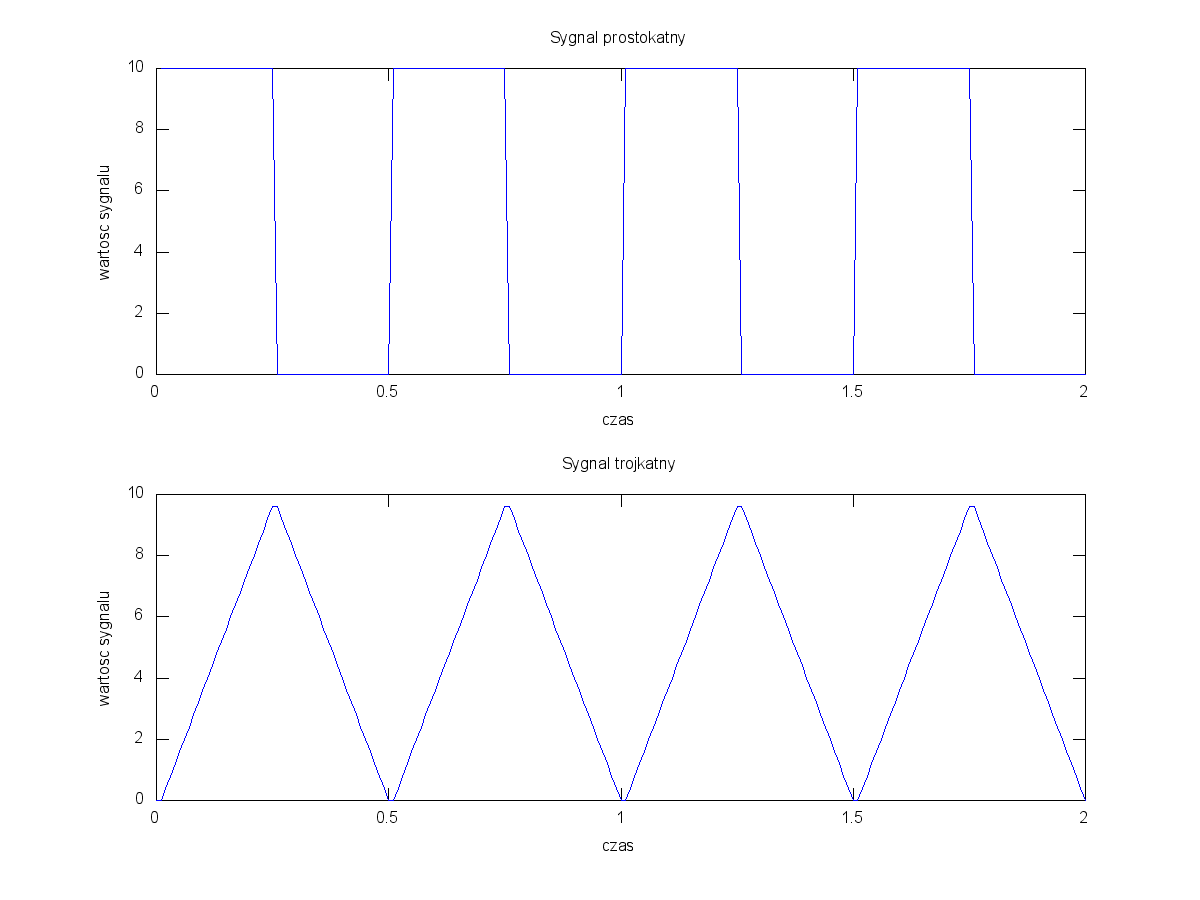
\includegraphics[scale=.5]{out/Figure1.png}
%       \caption{\label{wykres1}Badane sygnały.}
%     \end{center}
%   \end{figure}
% \end{landscape}
% Wykresy (end)
\end{document} 
